\documentclass{beamer}
\usetheme{Boadilla}
%==================================================
%Mypackages
\usepackage{epsf, amsmath, amssymb, epsfig, amsthm}
\usepackage{subfigure} % For subfigures
\usepackage{setspace} 
\usepackage{fancyhdr} 
\usepackage{eurosym}  %To write a Euro symbol
\usepackage[euler]{textgreek}
\usepackage[main=english,russian,spanish]{babel}
\usepackage[utf8]{inputenc}
\usepackage{graphicx}
\usepackage{float}
\usepackage{bbm}
\usepackage{cite}
\usepackage{listings}
\usepackage[font=small,labelfont=bf]{caption}
\usepackage{algorithm} 
\usepackage{algpseudocode} 
\lstset{
  basicstyle=\ttfamily,
  columns=fullflexible,
  frame=single,
  breaklines=true,
}
\hypersetup{colorlinks,urlcolor=blue}
\captionsetup[figure]{font=small}
\setbeamerfont{caption}{size=tiny}

%==================================================
%My commands: Define your commands here:

\begin{document}
\title{Planes, Trains, and Afflictions}
\subtitle{Agent-based modeling for the spread of disease through transportation networks}
\author{NS Group 3}
\institute[HSE]
{
  \inst{}%
  Faculty of Computer Science\\
  Higher School of Economics\\
  Moscow
}
\date{27 JUN 2020}
\begin{frame}
\titlepage
\end{frame}
\begin{frame}
\frametitle{Table of Contents}
\begin{itemize}
    \item Motivation
    \item Prior Research
    \item ABM Framework
    \item Examples
    \item Deep Dive: New York City (NYC) Subway
    \item Discussion
    \item Conclusion
    \item Credits
\end{itemize}
\end{frame}
\begin{frame}
\frametitle{Motivation}
Why were certain areas of NYC more affected by COVID-19?\\
How were the subways involved?\\
\begin{figure}
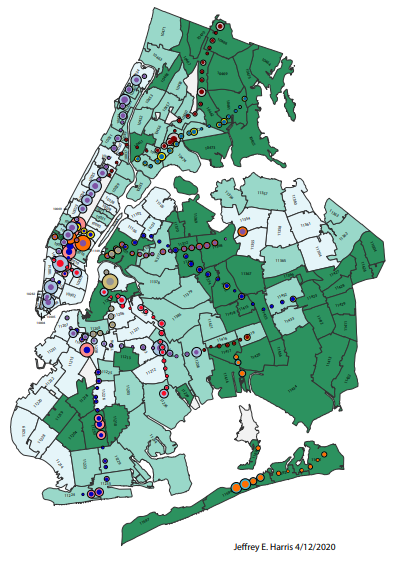
\includegraphics[width=4cm]{Scratch_Visuals/NYC_COVID_Subways_Jeff.png}%
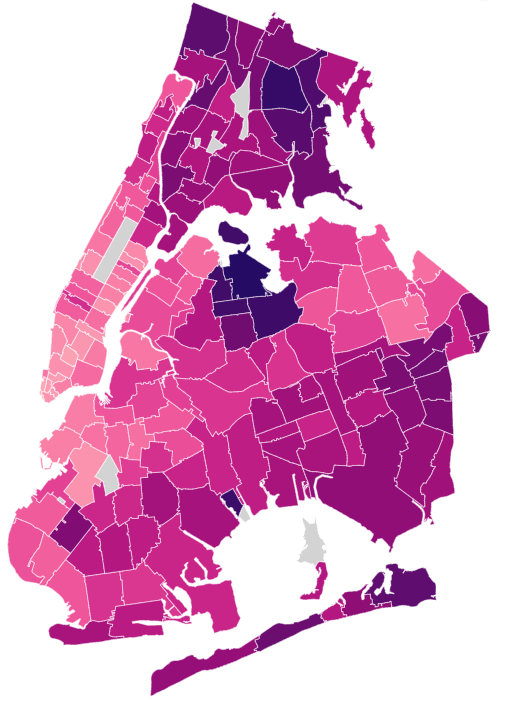
\includegraphics[width=4cm]{Scratch_Visuals/NYC_COVID_Case_Rate.png}
\caption{
Left: Case Rate And Subway On April 12, 2020 \cite{subway_epidemic_seed}\\
Right: NYC COVID Case Rate As Of June 23, 2020 \cite{nyc_health_covid_summary}
}
\end{figure}
\end{frame}
\begin{frame}
\frametitle{Prior Research (London Underground)}
Data: Oyster (Card), CASA (Timetable), PHE Data (Demographics)\\
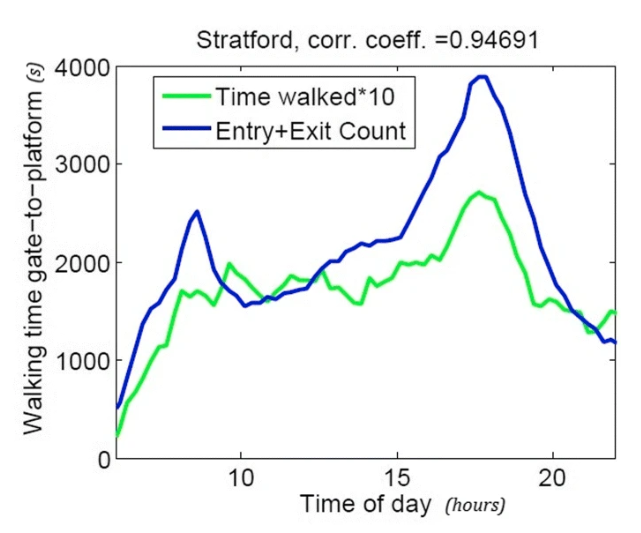
\includegraphics[width=0.5\textwidth]{Scratch_Visuals/London_Walking_time.png}%
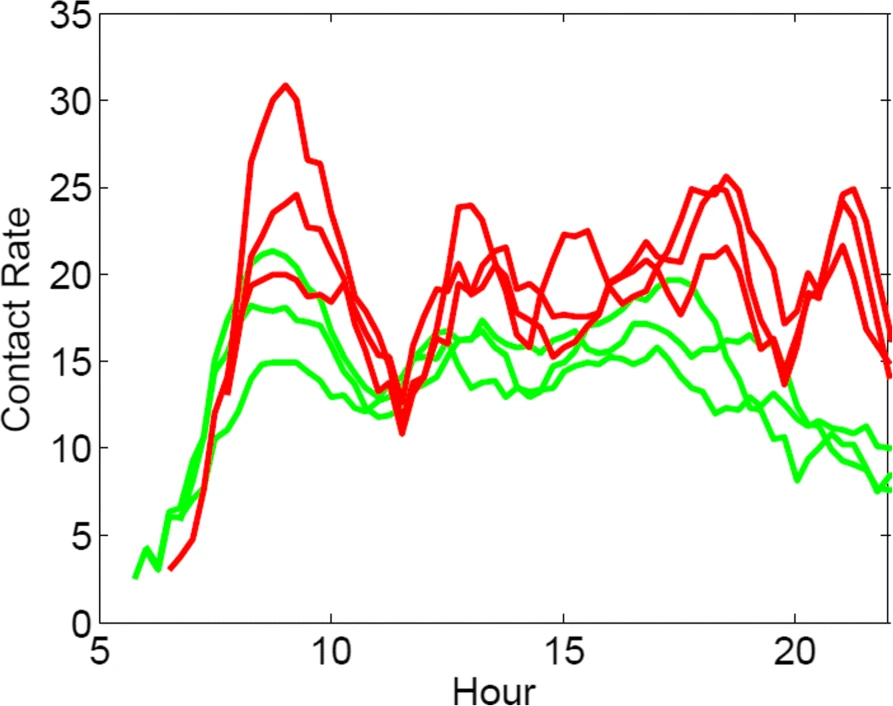
\includegraphics[width=0.5\textwidth]{Scratch_Visuals/London_Borough_Comparison.png}
\textit{Results show a correlation between the use of the underground and ILI cases in London, specifically they show that higher numbers of ILI cases arise in those boroughs where the population spend more time in the Underground and/or incur in a higher number of contacts when travelling.}
 \cite{gosce_johansson_2018}
\end{frame}
\begin{frame}
\frametitle{COVID in London}
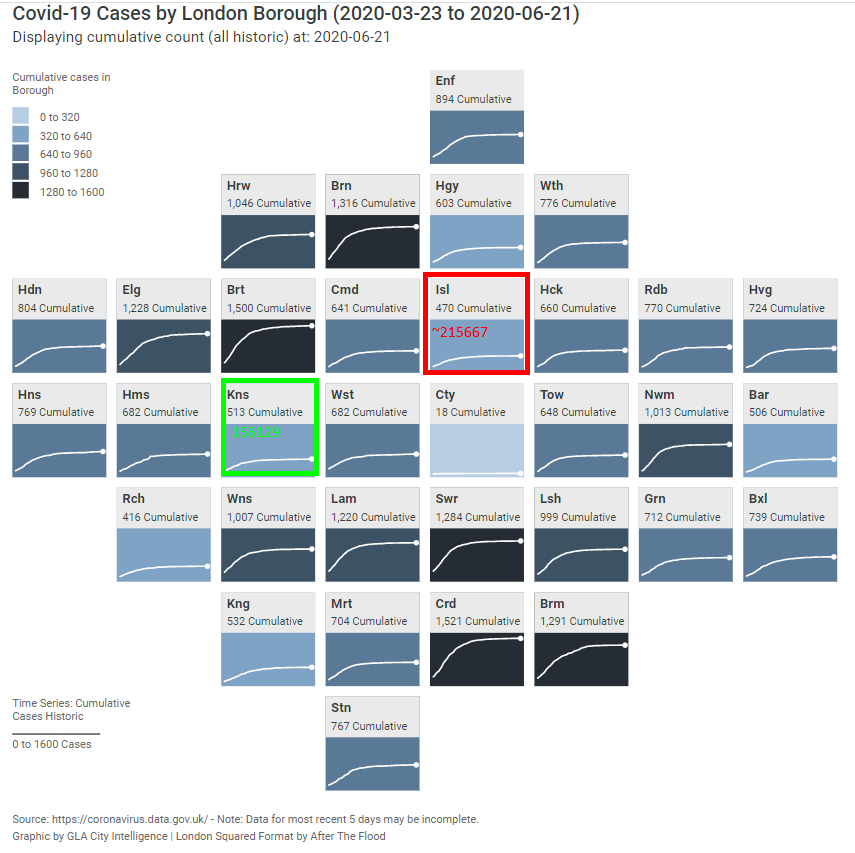
\includegraphics[width=0.7\textwidth]{Scratch_Visuals/London_Covid_Adapted.png}
\textit{Speaker's Remark: Boroughs of NY != Boroughs of London}
\end{frame}
\begin{frame}
\frametitle{Prior Research (Singapore Buses)}
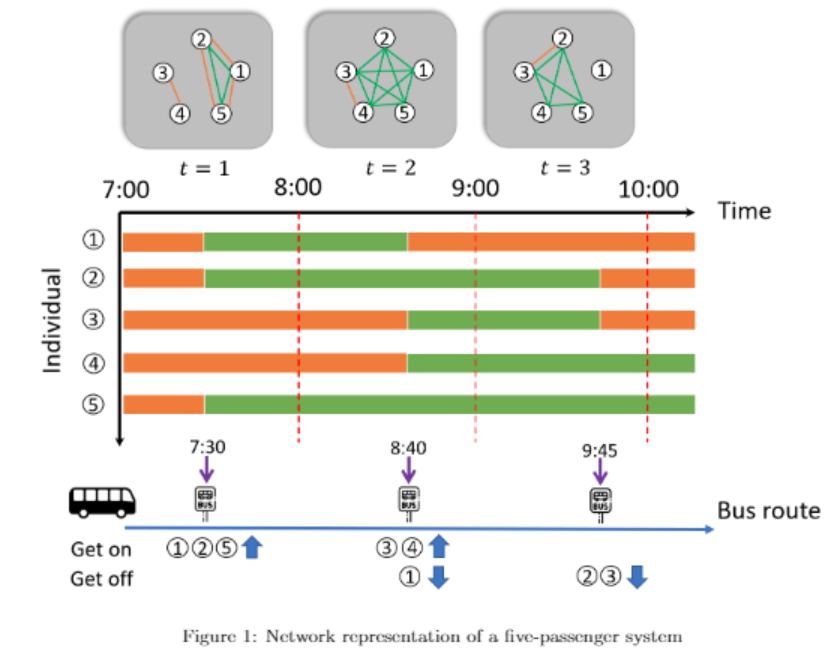
\includegraphics[width=0.5\textwidth]{Scratch_Visuals/Singapore_1.png}%
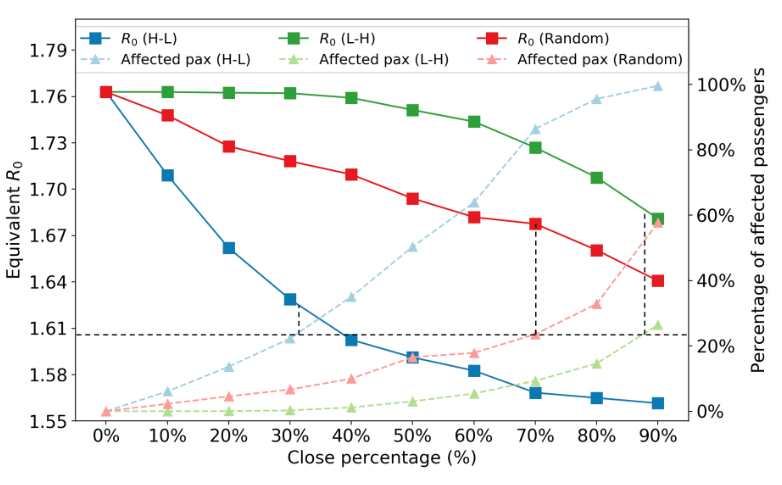
\includegraphics[width=0.5\textwidth]{Scratch_Visuals/Singapore_2.png}
\textit{The direct contact in trains is, however, difficult to obtain from smart card data because the transactions are recorded at the station level}
\cite{singapore_bus_2020}
\textit{Speaker's note:\\
- We show these things not to embarrass ourselves, but the depth of research available even just looking at one system.
- List some other research
}
\end{frame}
\begin{frame}
\frametitle{ABM Framework}
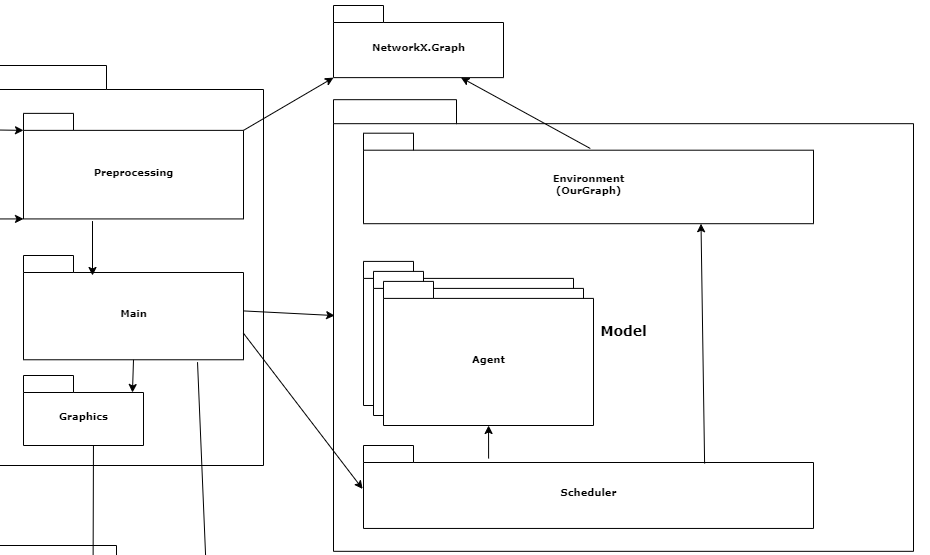
\includegraphics[width=1.0\textwidth]{Scratch_Visuals/covid_framework_summary.png}
Components: Python, MESA, Networkx\\
Base Classes: \href{https://github.com/cheung-ho-lum/NS_Epidemics_ABM_Approach/blob/master/Report/Design_doc_for_expansion_of_subway_model.pdf}{Transportation Model, SEIR Agent}
\end{frame}
\begin{frame}{Embedded Animation}
\frametitle{Simple Geometries}
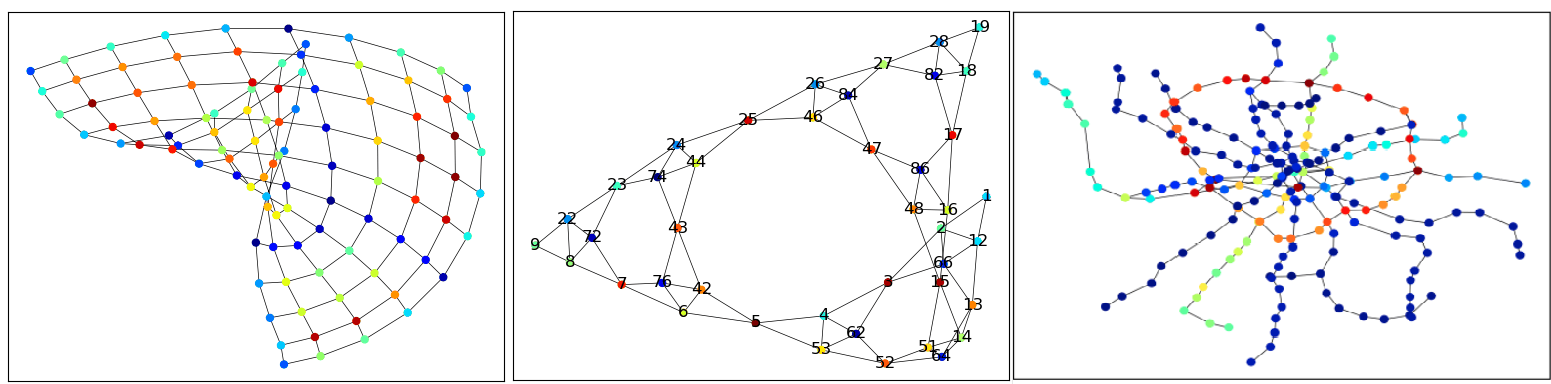
\includegraphics[width=1.0\textwidth]{Scratch_Visuals/geometries_example.png}
\begin{itemize}
    \item \href{https://github.com/cheung-ho-lum/NS_Epidemics_ABM_Approach/blob/master/Repository/Visualizations/infection_timelapse_grid_01.gif}{Grid}
    \item \href{https://github.com/cheung-ho-lum/NS_Epidemics_ABM_Approach/blob/master/Repository/Visualizations/infection_timelapse_sierpinski_01.gif}{Sierpinski's Triangle}
    \item \href{https://github.com/cheung-ho-lum/NS_Epidemics_ABM_Approach/blob/master/Repository/Visualizations/infection_timelapse_moscow.gif}{Moscow}
\end{itemize}
\end{frame}


\begin{frame}
\frametitle{World Airline Network (Passenger Flow) - Challenges}
Obtaining accurate data bout world passenger flow is a bit of callenge, one has 3 options:
\begin{enumerate}
	\item Pay for it
	\item Using superior math to extrapolate or estimate
	\item Extrapolate based on what I know; We obted for option 3 
\end{enumerate}
\end{frame}
\begin{frame}
\frametitle{Algorithm 1 to estimate WAN (Passenger Flow)}
\begin{enumerate}
	\item Find total number of passengers going through a specific airport
	\item Total number of destinations from said airport
	\item Ratio of traffic from each airport
	\item Split population of passengers into various destinations based on ratio 
\end{enumerate}
Major challenge with this is the fact that we need to find data to answer each of these questions  in order to make an estimate (ratios data)
\end{frame}

\begin{frame}
\frametitle{Algorithm 2 to estimate WAN (Passenger Flow)}
Using Data from Wikipedia and Openflights
\begin{enumerate}
	\item Get the total population of data passengers that go through a specific airport.
	\item Using HITS algorithm on airport pairs.
	\item Split population of passengers into various destinations based on hubs obtained from HITS
\end{enumerate}
Major challenge with this is the fact that the graph is undirected hence the HITS results were unreliable. Also if the data was split into major known hubs the data returned the same value from HITS.
\end{frame}

\begin{frame}
\frametitle{World Airline Network (Passenger Flow)  Algorithm}
\end{frame}



\begin{frame}
\frametitle{Madrid Commuter Trains (Central Hubs)}
How important are central transportation hubs to disease spread?\linebreak
\linebreak
Data Sources:
\begin{itemize}
	\item Madrid Renfe GTFS: \url{https://crtm.maps.arcgis.com/home/item.html?id=1a25440bf66f499bae2657ec7fb40144}
	\item Madrid Renfe Turnstile data: \url{https://data.renfe.com/dataset/volumen-de-viajeros-por-franja-horaria-madrid}
\end{itemize}
\end{frame}
\begin{frame}
\frametitle{Madrid Commuter Trains}
\begin{figure}
	\centering
	\begin{subfigure}
		\centering
		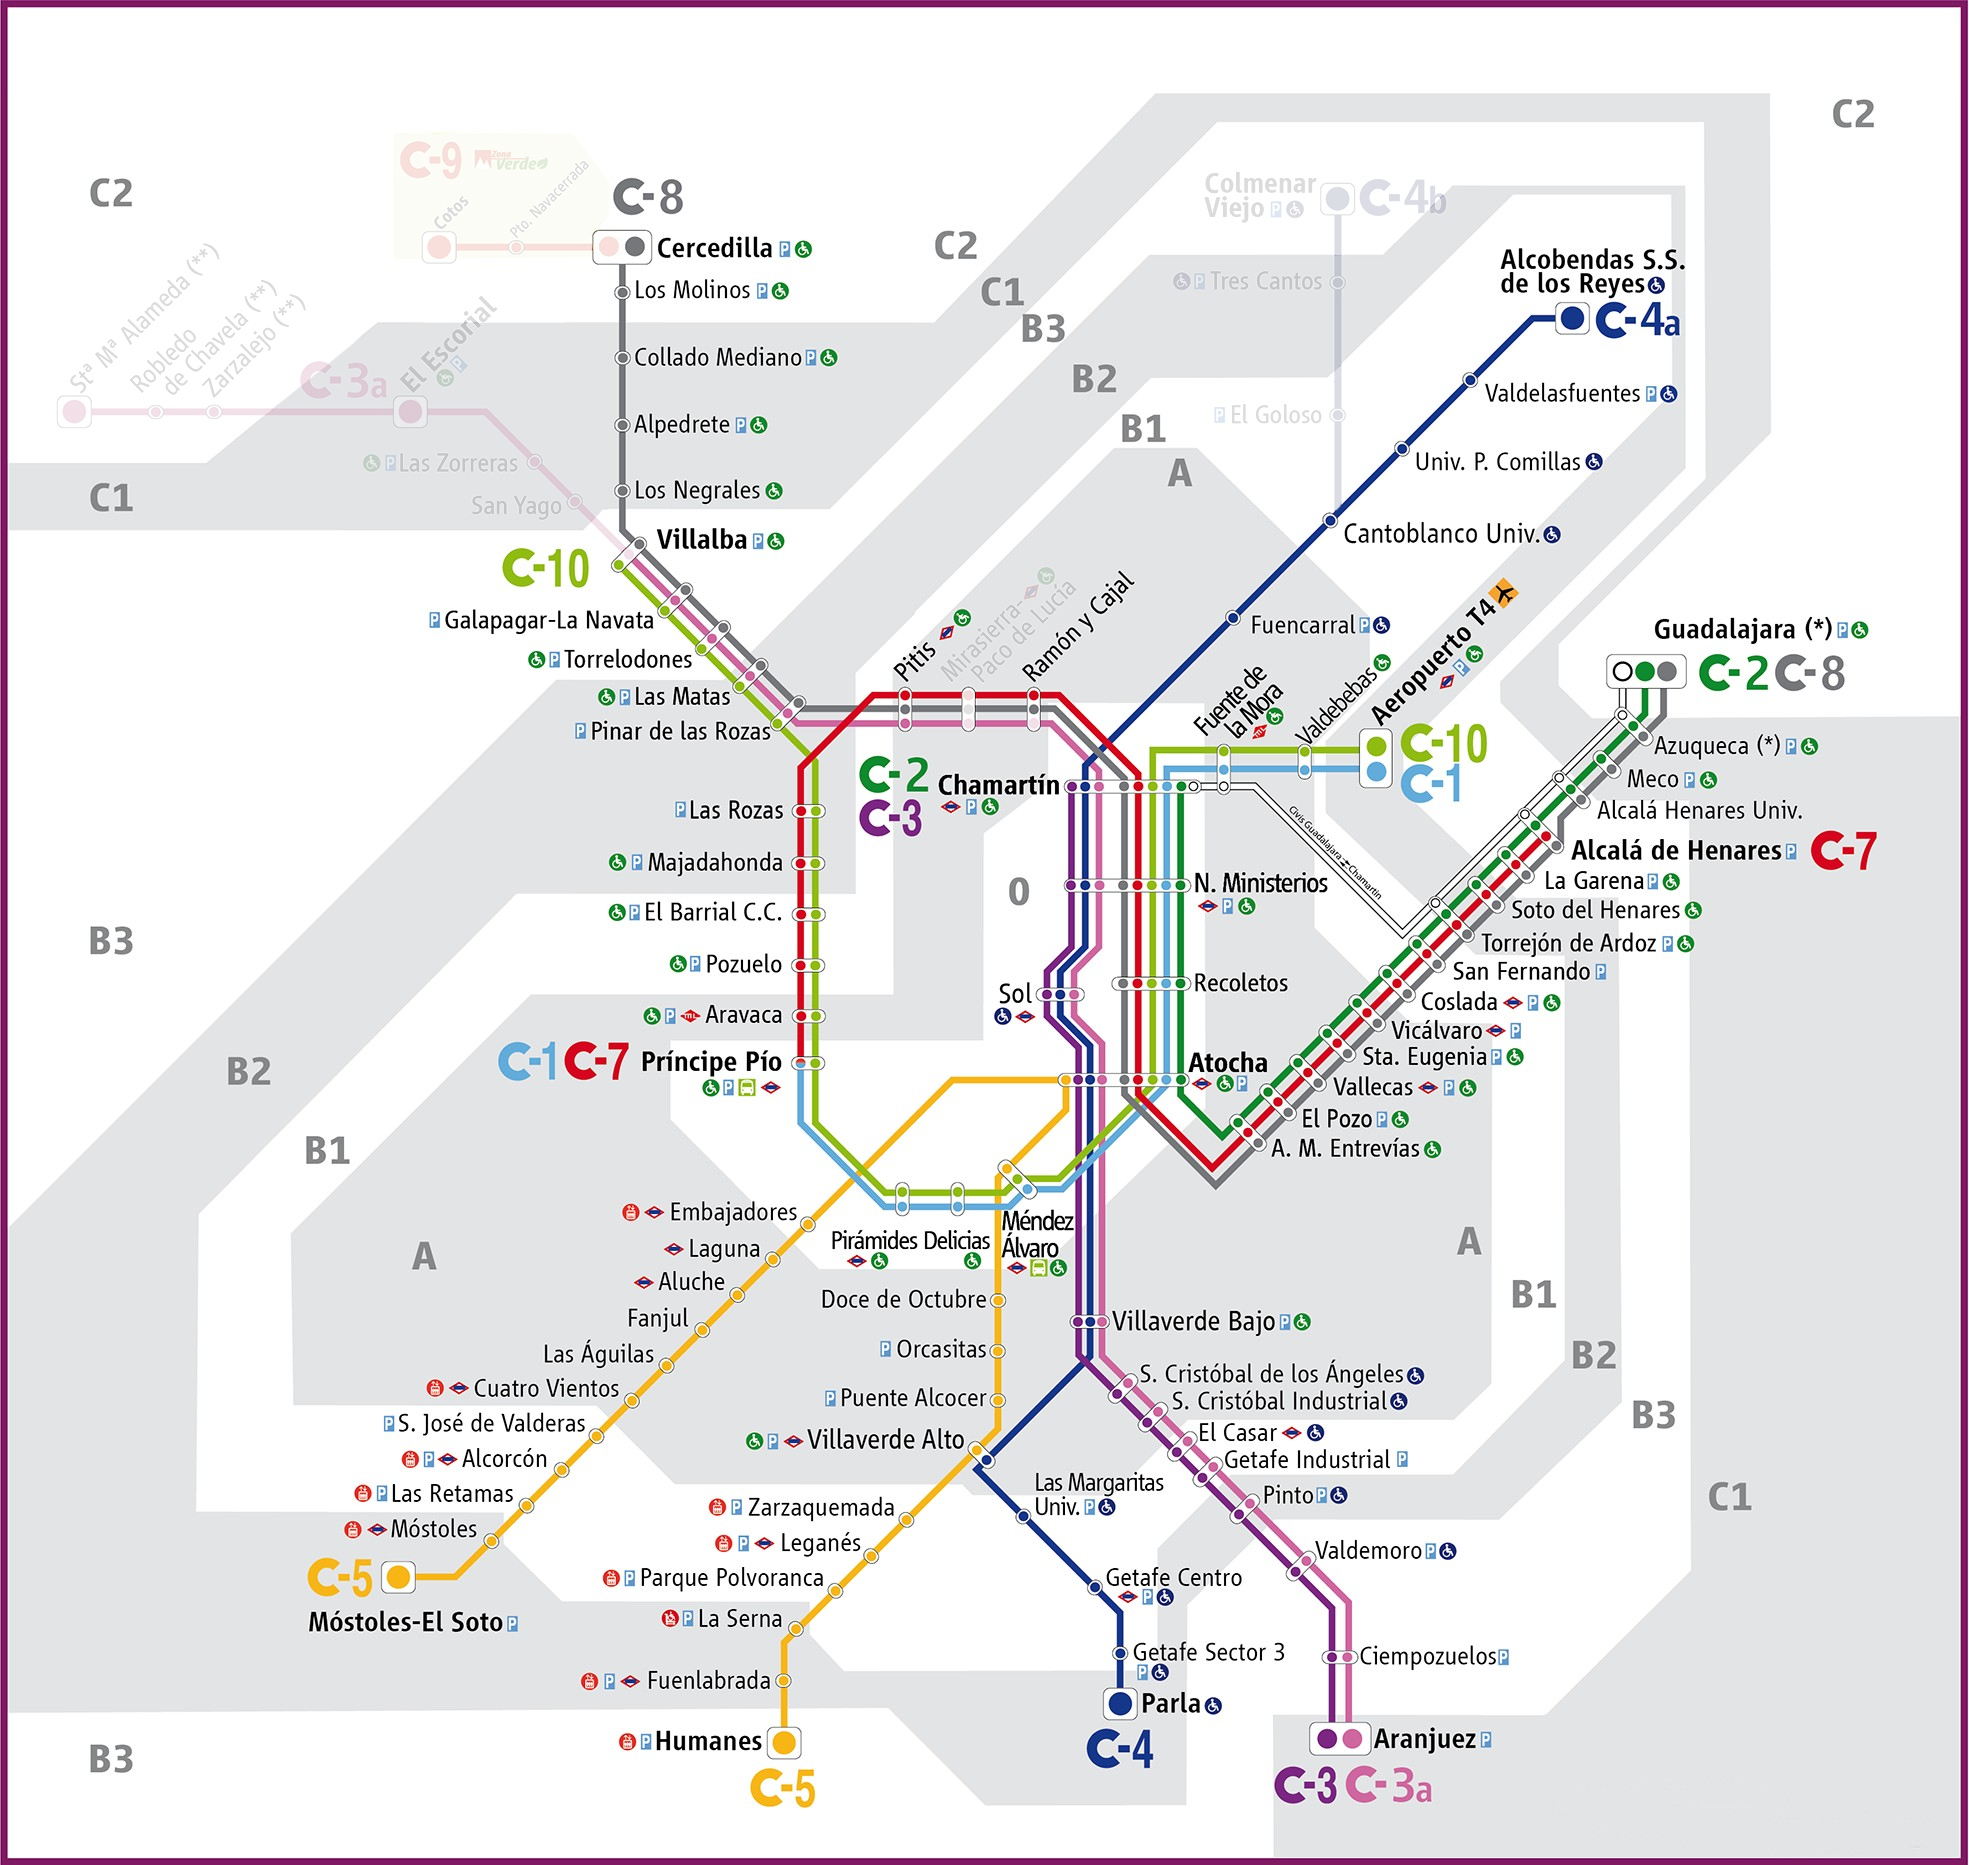
\includegraphics[width=.4\linewidth]{Scratch_Visuals/madrid-cercanias-map-fix.png}
	\end{subfigure}%
	\begin{subfigure}
		\centering
		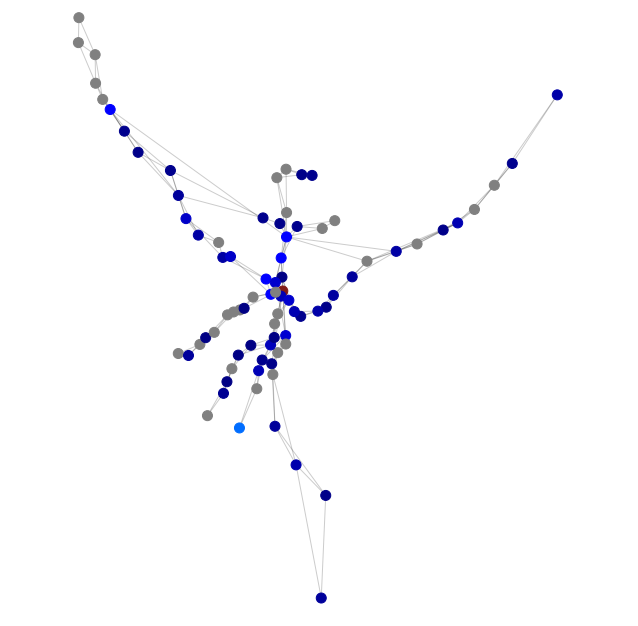
\includegraphics[width=.4\linewidth]{Scratch_Visuals/madrid-cercanias-map-py.png}
	\end{subfigure}
	\caption{Madrid Cercanias map 2020 (urban trains)}
\end{figure}
\end{frame}
\begin{frame}
\frametitle{Madrid Commuter Trains}
Method: Agent Based Model (ABM)\linebreak
Agents: passengers\linebreak
Flow based on weights $w$ which depend on the turnstiles data: \textit{in-weight} and \textit{out-weight} (incoming and outcoming passengers respectively).
\end{frame}
\begin{frame}
\frametitle{Madrid Commuter Trains - Passengers flow}
At each time step $t$...\linebreak
\linebreak
$N$ passengers join the network randomly:
\begin{enumerate}
	\item Join at a random time.
	\item Origin station depending on the \textit{in-weight}.
	\item Platform choice based on the weight of the next platforms.
	\item The passengers wait in the platform until a train arrives.
\end{enumerate}
Passengers who are in a train:
\begin{itemize}
\item Leave the network (destination arrival) depending on the \textit{out-weight} of the station.
\item Leave the train and go to another platform depending on the weights of each platform.
\end{itemize}
\end{frame}
\begin{frame}
\frametitle{Madrid Commuter Trains - Parameters}
In order to simulate the spread of an infection:
\begin{itemize}
	\item Passengers (in a day): $500,000$.
	\item Infected passengers: $50,000$ ($10\%$ of them).
	\item Infection probability: $0.005$.
\end{itemize}
On average, an infected passenger will infect to other $5.04$ people.
\end{frame}
\begin{frame}
\frametitle{Madrid Commuter Trains - Results}
\begin{figure}
	\centering
	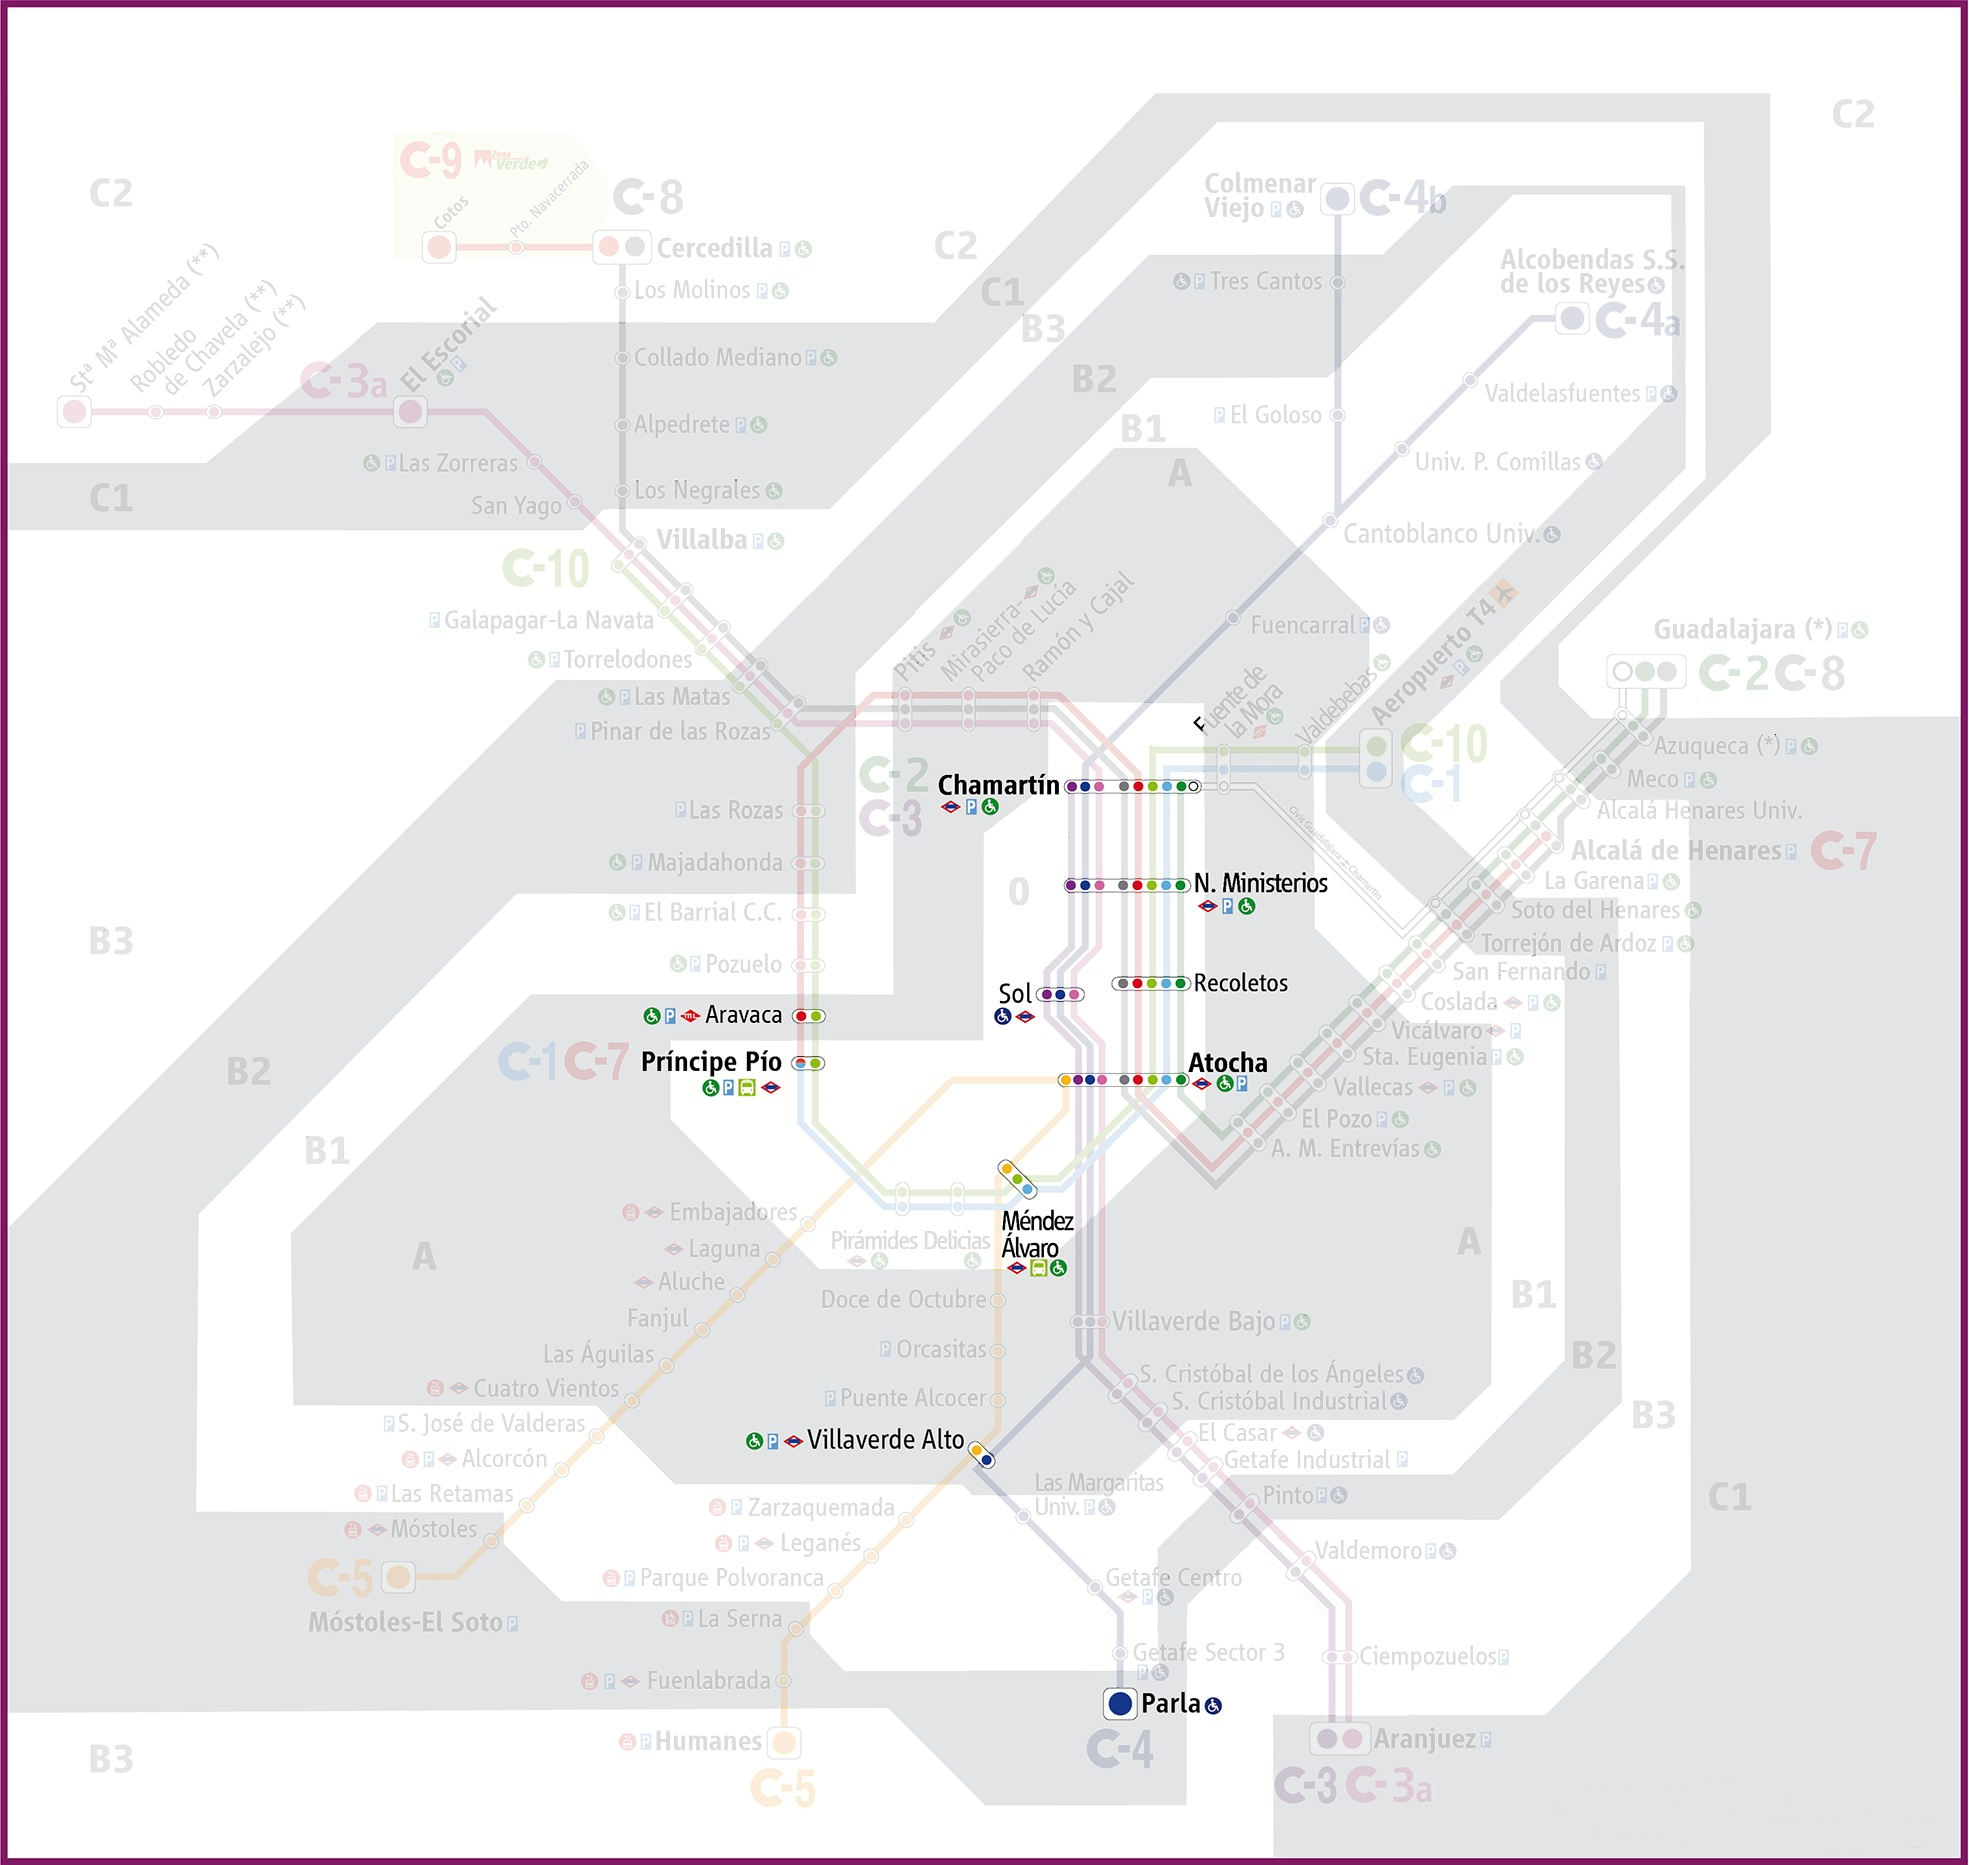
\includegraphics[width=.5\linewidth]{Scratch_Visuals/madrid-cercanias-map-top10.png}
	\caption{Top 10 stations with more infections}
\end{figure}
\end{frame}
\begin{frame}
\frametitle{Madrid Commuter Trains - Results}
\begin{figure}
	\centering
	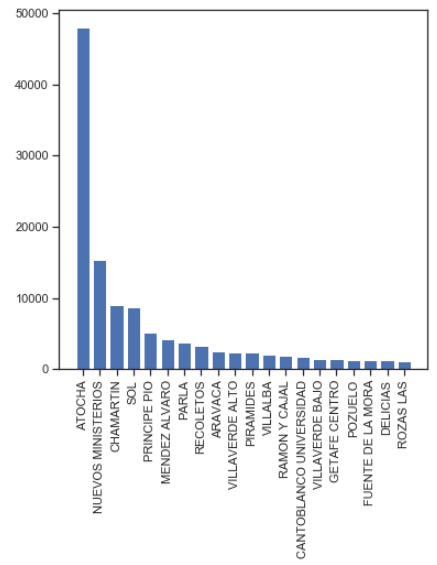
\includegraphics[width=.4\linewidth]{Scratch_Visuals/madrid-cercanias-stats-top20.png}
	\caption{Top 20 stations with more infections}
\end{figure}
\end{frame}
\begin{frame}
\frametitle{Madrid Commuter Trains - Results}
\begin{figure}
\centering
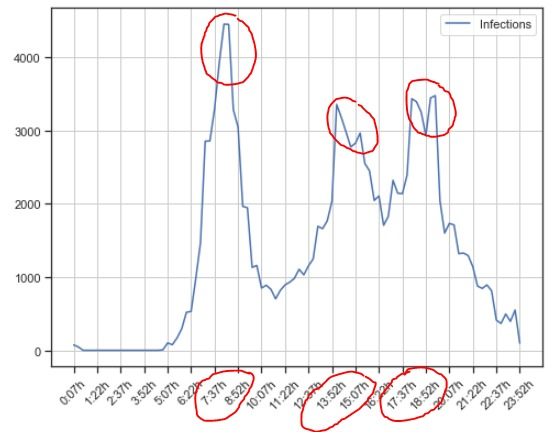
\includegraphics[width=.6\linewidth]{Scratch_Visuals/madrid-infection-timeline.jpg}
\caption{Infections in the whole network during a day.}
\end{figure}
\end{frame}
\begin{frame}
\frametitle{Madrid Commuter Trains - Results}
\begin{figure}
	\centering
	\begin{subfigure}
		\centering
		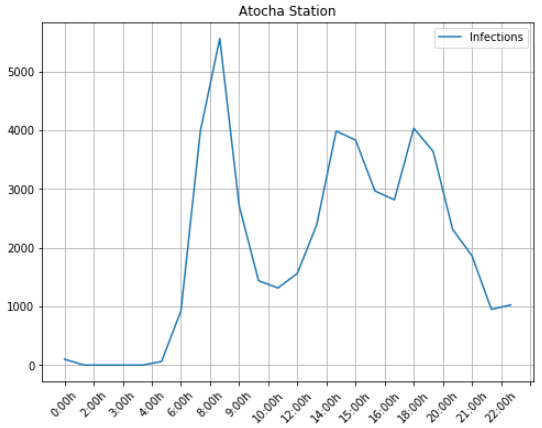
\includegraphics[width=.4\linewidth]{Scratch_Visuals/madrid-infection-timeline-atocha.png}
	\end{subfigure}%
	\begin{subfigure}
		\centering
		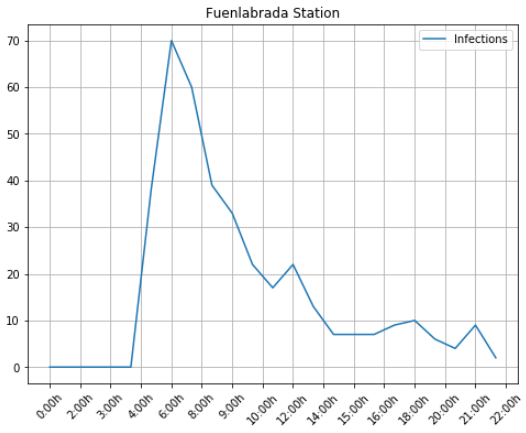
\includegraphics[width=.4\linewidth]{Scratch_Visuals/madrid-infection-timeline-fuenlabrada.png}
	\end{subfigure}
	\caption{Infections in a central hub (left) and a station in a suburb (right).}
\end{figure}
\end{frame}


\begin{frame}
\frametitle{NYC Demographics And COVID Timeline
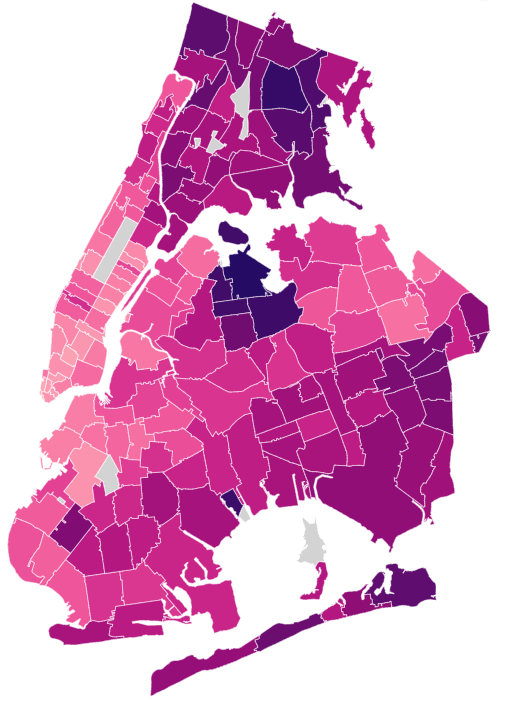
\includegraphics[width=1cm]{Scratch_Visuals/NYC_COVID_Case_Rate.png}
}
\textit{NYC residents working in Manhattan primarily travel by subway. This is
also true for residents of the Bronx, Brooklyn, and Queens\cite{nyc_commuting}}
\begin{itemize}
	\item March 9 - Mayor holds press conference and notes that there have been 16 confirmed cases. (106 cases)
	\item March 12 - Mayor declares a local state of emergency. (687 cases)
	\item March 15 - Schools officially close. (2,986 cases)
\end{itemize}
Borough - A geographical region. NYC has 5 boroughs. \\
MODZCTA - Modified Zip Code Tabulation Areas. $\propto$ postal codes.\\
\end{frame}
\begin{frame}
\frametitle{Subway Systems}
Complex, Station, Line, Route
\begin{figure}
    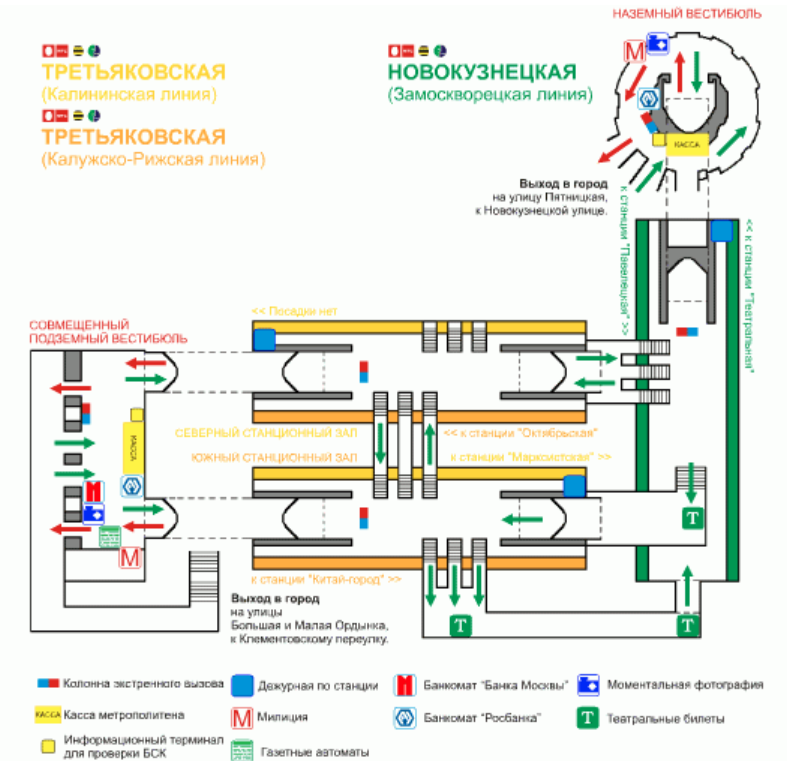
\includegraphics[width=6cm]{Scratch_Visuals/Novokuznetskaya.png}
    \caption{Floor Plan of Novokuznetskaya Metro Station \cite{Novokuznetskaya}}
\end{figure}
\end{frame}
\begin{frame}[fragile, shrink=5]
\frametitle{NYC Subway Data}
Stations, Map, Turnstiles (GTFS not considered)
\begin{figure}
    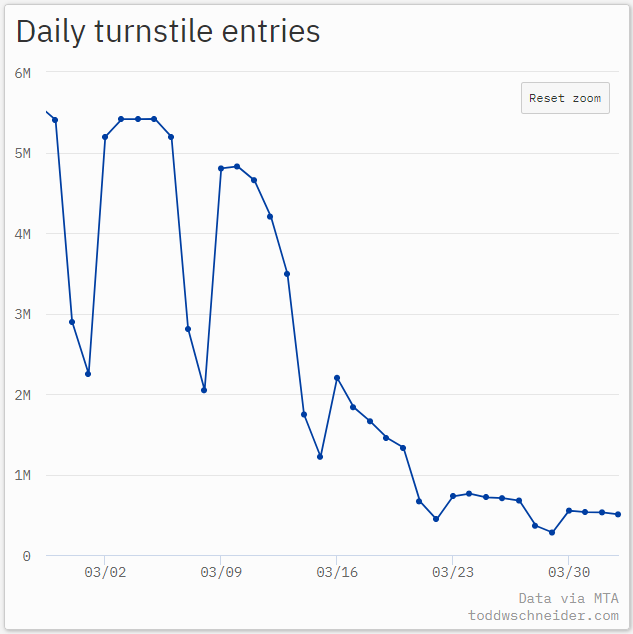
\includegraphics[width=6cm]{Scratch_Visuals/schneider_ridership.png}
    \caption{NYC Subway daily turnstile entries for March 2020 \cite{toddwschneider}}
\end{figure}
\begin{verbatim}
167,167,A32,IND,8th Av - Fulton St,W 4 St,M,A C E...
167,167,D20,IND,6th Av - Culver,W 4 St,M,B D F M...
\end{verbatim}
\end{frame}
\begin{frame}[shrink=5]
\frametitle{NYC Subway Modeling}
\begin{algorithm}[H]
\caption{Simulation of Disease Spread on Subways}\label{euclid}
\begin{algorithmic}[1]
\For{$i=1; i < TIMESPAN; i++$}
    \State Check conditions (i, number of infected) to see if we should deploy COUNTERMEASURES
    \For{Station in SubwayModel.Environment.Nodes}
        \State Calculate 'Local Exposure' from infected and commute time.
        \State Calculate 'Route Exposure' from infected on the same route.
        \State Calculate 'General Exposure' due to city-wide infected.
        \State Update 'Exposure' at station based on above conditions
    \EndFor
    \For{Agent in SubwayNetwork.Agents}
        \State Get 'Exposure' At Location
        \State Get City-wide COUNTERMEASURES
        \State Get Percentage of commuters
        \State Calculate SEIR beta and gamma based on conditions
        \State Update SEIR numbers
    \EndFor
\EndFor
\end{algorithmic}
\end{algorithm}
Subway Agent - SEIR Agent with additional exposure based on location. \\
Subway Graph - Nodes $\propto$ Stations, Edges $\propto$ \textbf{Lines, Complex}, Route Lookup.
\end{frame}
\begin{frame}
\frametitle{NYC Model Parameters, Hyper-parameters}
Default SEIR Rates: $\beta,\alpha,\gamma$ = 1.75, 0.20, 0.50 \\
Countermeasures: Isolation, Recommendation, Awareness: = 5000, 500, 500 \\
\textit{Defiance}: 10\% Local, 25\% Global \\
\textit{Global Exposure}: 0.7 \\
\textit{Commute Time}: ~Squared shortest path from Grand Central or Times Square \\
\end{frame}
\begin{frame}
\frametitle{Compartmental Modeling Results (NYC)}
\begin{figure}
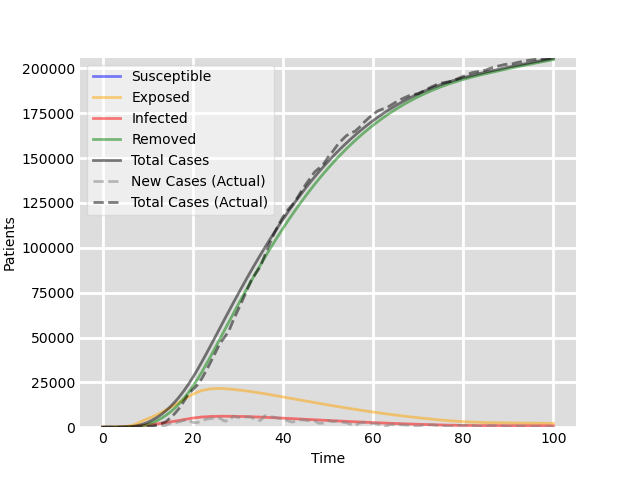
\includegraphics[width=0.8\textwidth]{Scratch_Visuals/SEIR_Curve_NYC_3.png}
\caption{SEIR Fitting to NYC Case Total. \textit{MAPE ($t \geq 30$): 0.0145}}
\end{figure}
\end{frame}
\begin{frame}
\frametitle{Results by MODZCTA (NYC)}
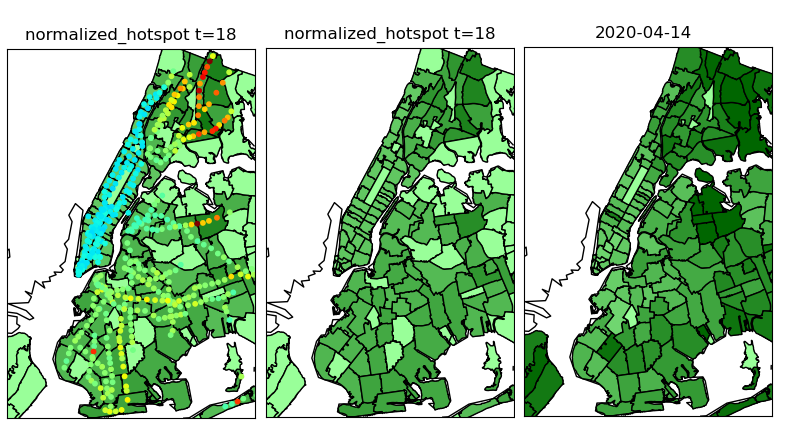
\includegraphics[width=1.0\textwidth]{Scratch_Visuals/NYC_Geo_Fitting.png}
\href{https://github.com/cheung-ho-lum/NS_Epidemics_ABM_Approach/blob/master/Repository/Visualizations/infection_timelapse_NYC_3.gif}{New York City Timelapse}
\end{frame}
\begin{frame}
\frametitle{Discussion}
All models are wrong!\\
\begin{itemize}
    \item Passenger Flow
    \item Outer suburbs phenomenon exists
    \item Simple GDP/capita data
    \item Erase some of these stupid parameters
\end{itemize}
\end{frame}
\begin{frame}
\frametitle{Conclusions}
\begin{itemize}
    \item Determining passenger flow is a difficult problem for all transportation networks at all granularities.
    \item 
    \item 
\end{itemize}
\end{frame}
\begin{frame}
\frametitle{Credits, Links, References}
Frank Acquaye - WAN, Passenger Flow\\
Ho Lum Cheung - NYC, Organization, Research, Testing\\
Dimas Muñoz-Montesinos - Madrid, Hotspots\\
Elie Wanko - Theory, Consulting\\
github link
references used in slides
\bibliography{bib_file}{}
\bibliographystyle{plain}
\end{frame}
\end{document}